\section{Sinusoidal $f(t)$ with normal box kernel}
This report analyzes how the convolution of a sinusoidal signal with a rectangular kernel depends on various parameters. We consider the input signal $f(t) = A\sin(\omega t + \phi)$ and the rectangular kernel $h(t) = 1$ for $-T \leq t \leq T$ and 0 elsewhere.

\subsection{Analytical Solution}
The convolution of $f(t)$ with $h(t)$ is given by:
\begin{equation}
y(t) = (f * h)(t) = \int_{-\infty}^{\infty} f(\tau)h(t-\tau)d\tau
\end{equation}

For our specific functions, this simplifies to:
\begin{align}
y(t) &= \int_{t-T}^{t+T} A\sin(\omega\tau + \phi)d\tau\\
&= \frac{A}{\omega}[\cos(\omega(t-T) + \phi) - \cos(\omega(t+T) + \phi)]\\
&= \frac{2A}{\omega}\sin(\omega T)\sin(\omega t + \phi)
\end{align}

\subsection{Parameter Dependencies}

\subsubsection{Effect of Input Signal Amplitude}
The amplitude $A$ of the input signal linearly scales the output amplitude. As shown in Figure \ref{fig:amplitude}, the convolution output preserves this linear relationship, with the output amplitude being $\frac{2A}{\omega}\sin(\omega T)$ times the input amplitude.

\begin{figure}[H]
    \centering
    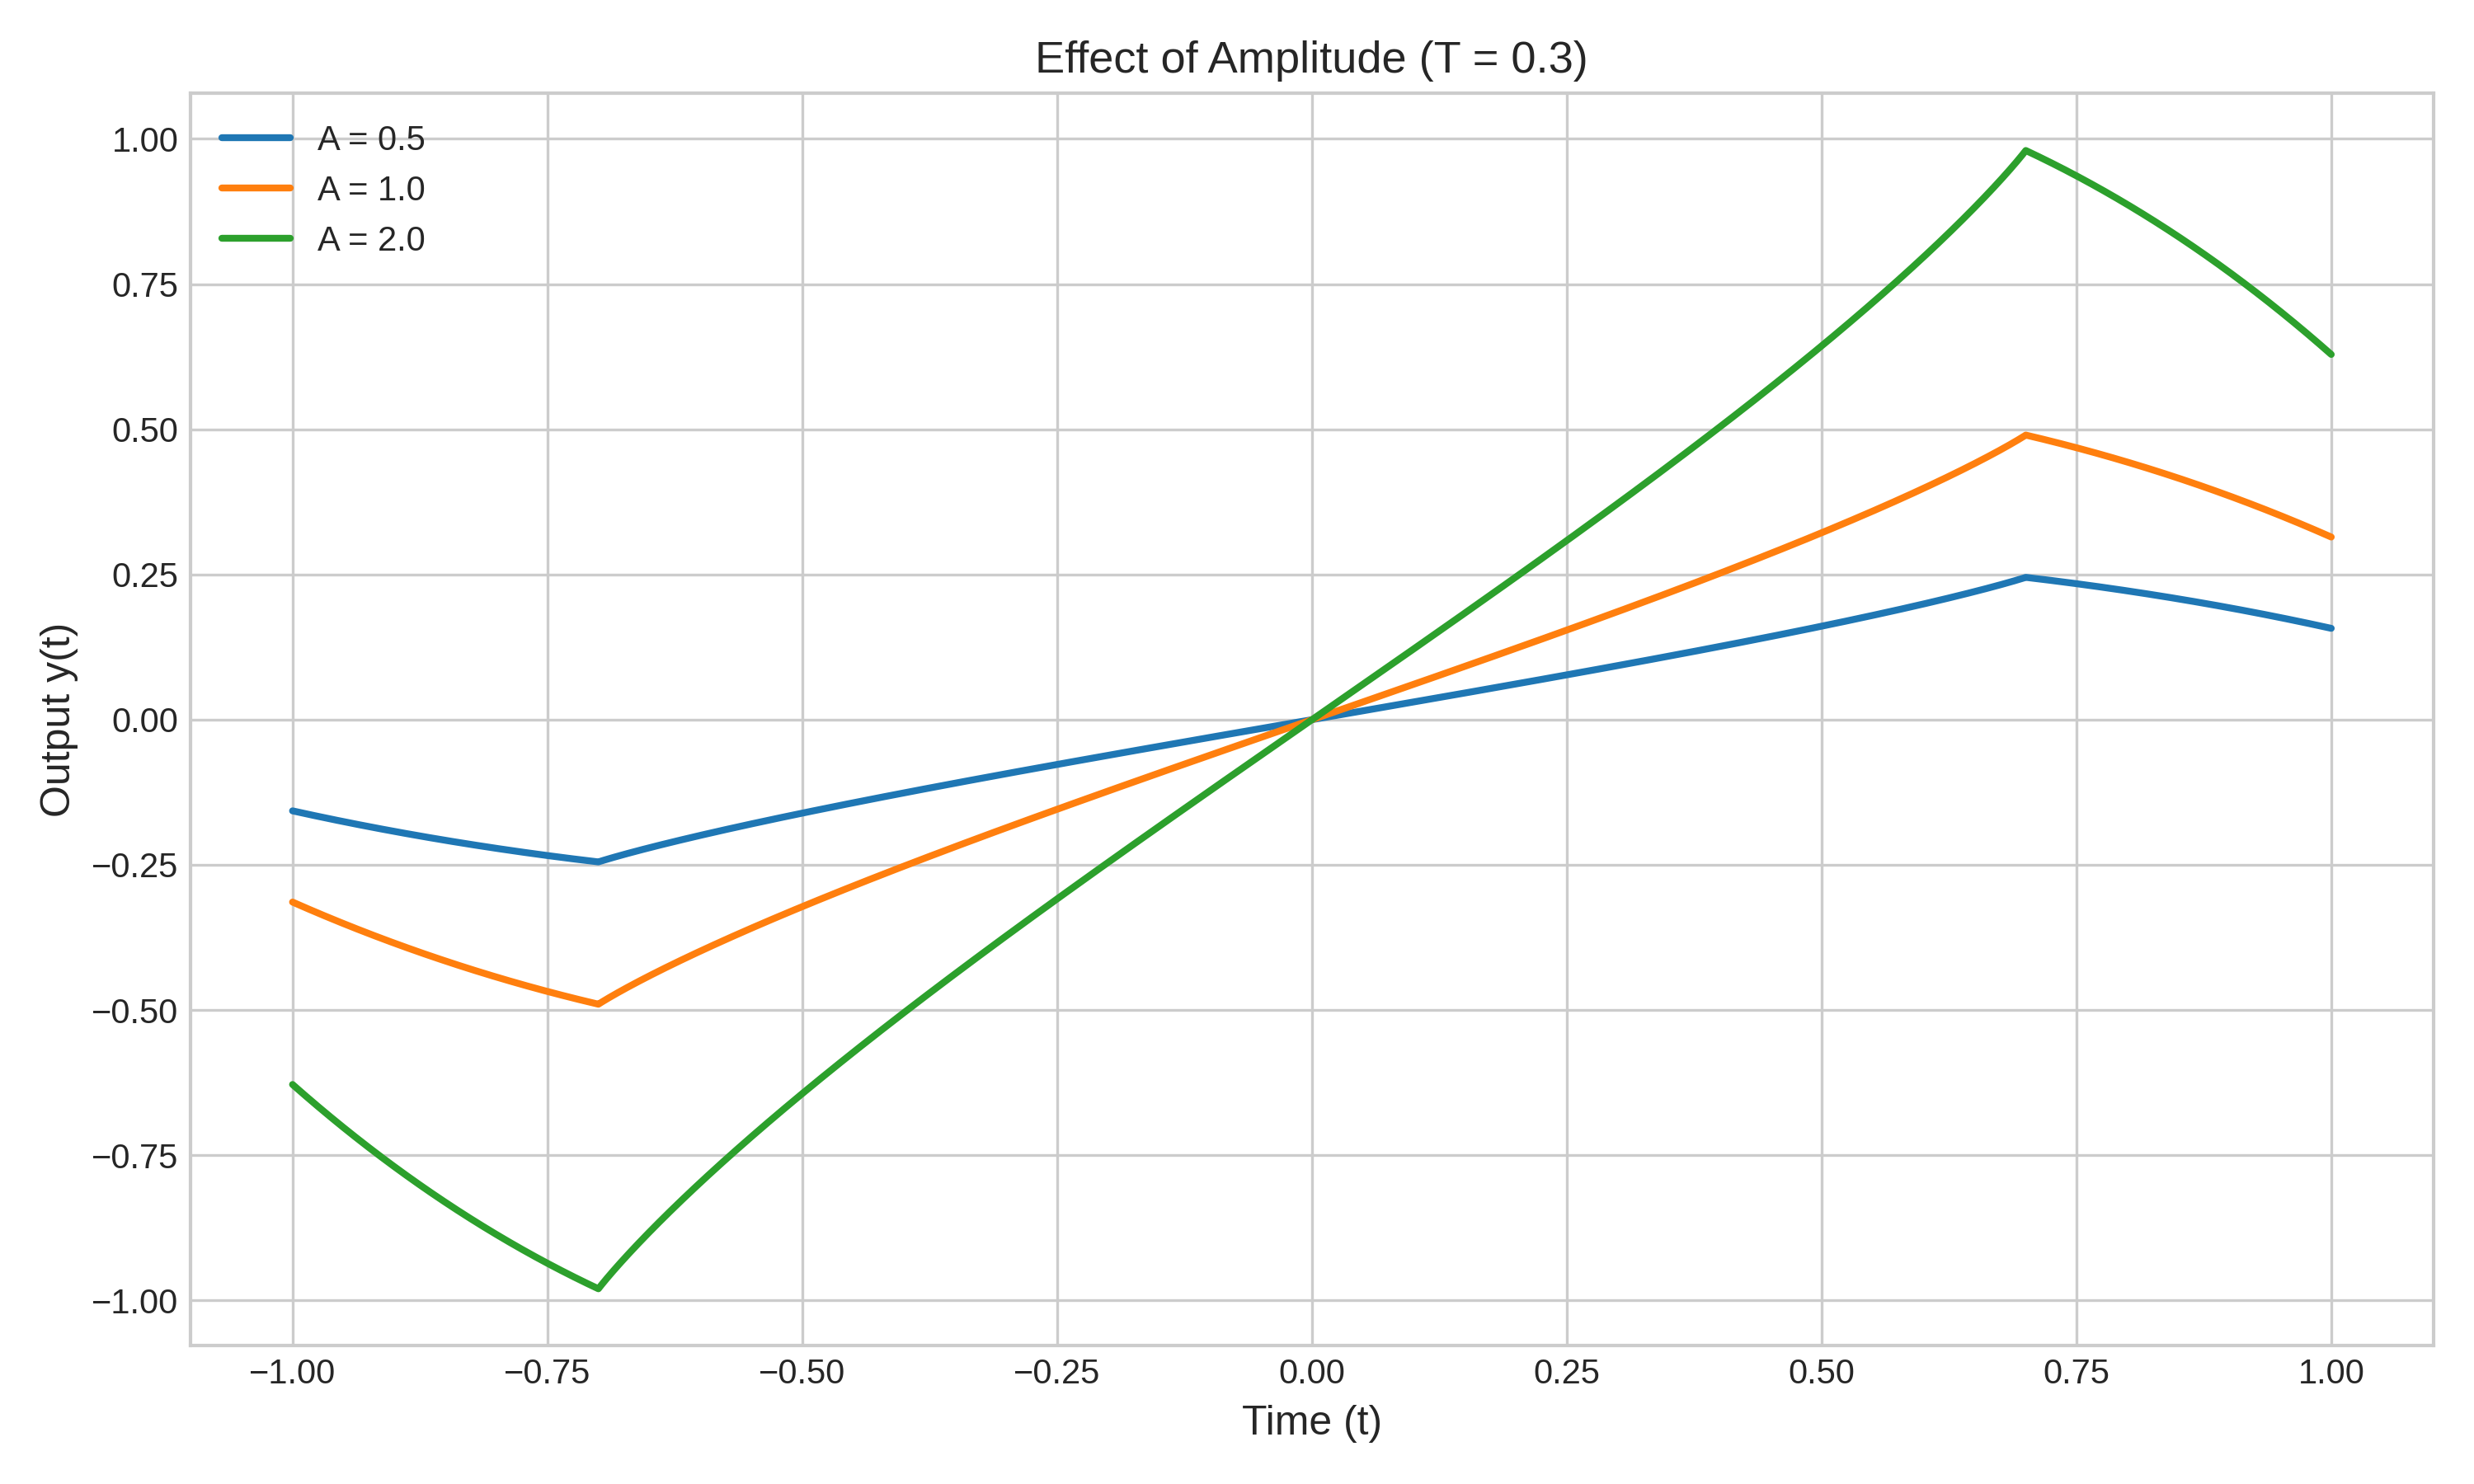
\includegraphics[width=0.8\textwidth]{codes/codes_sin_1_and_arcsin/figures/amplitude_effect.png}
    \caption{Effect of varying input signal amplitude on convolution output.}
    \label{fig:amplitude}
\end{figure}

\subsubsection{Effect of Input Signal Frequency}
The frequency $\omega$ affects the convolution in two ways:
\begin{enumerate}
    \item It determines the oscillation rate of the output signal
    \item It scales the output amplitude through the factor $\frac{2\sin(\omega T)}{\omega}$
\end{enumerate}

Higher frequencies generally result in smaller amplitudes due to the $\frac{1}{\omega}$ in the amplitude factor, as demonstrated in Figure \ref{fig:frequency}.

\begin{figure}[H]
    \centering
    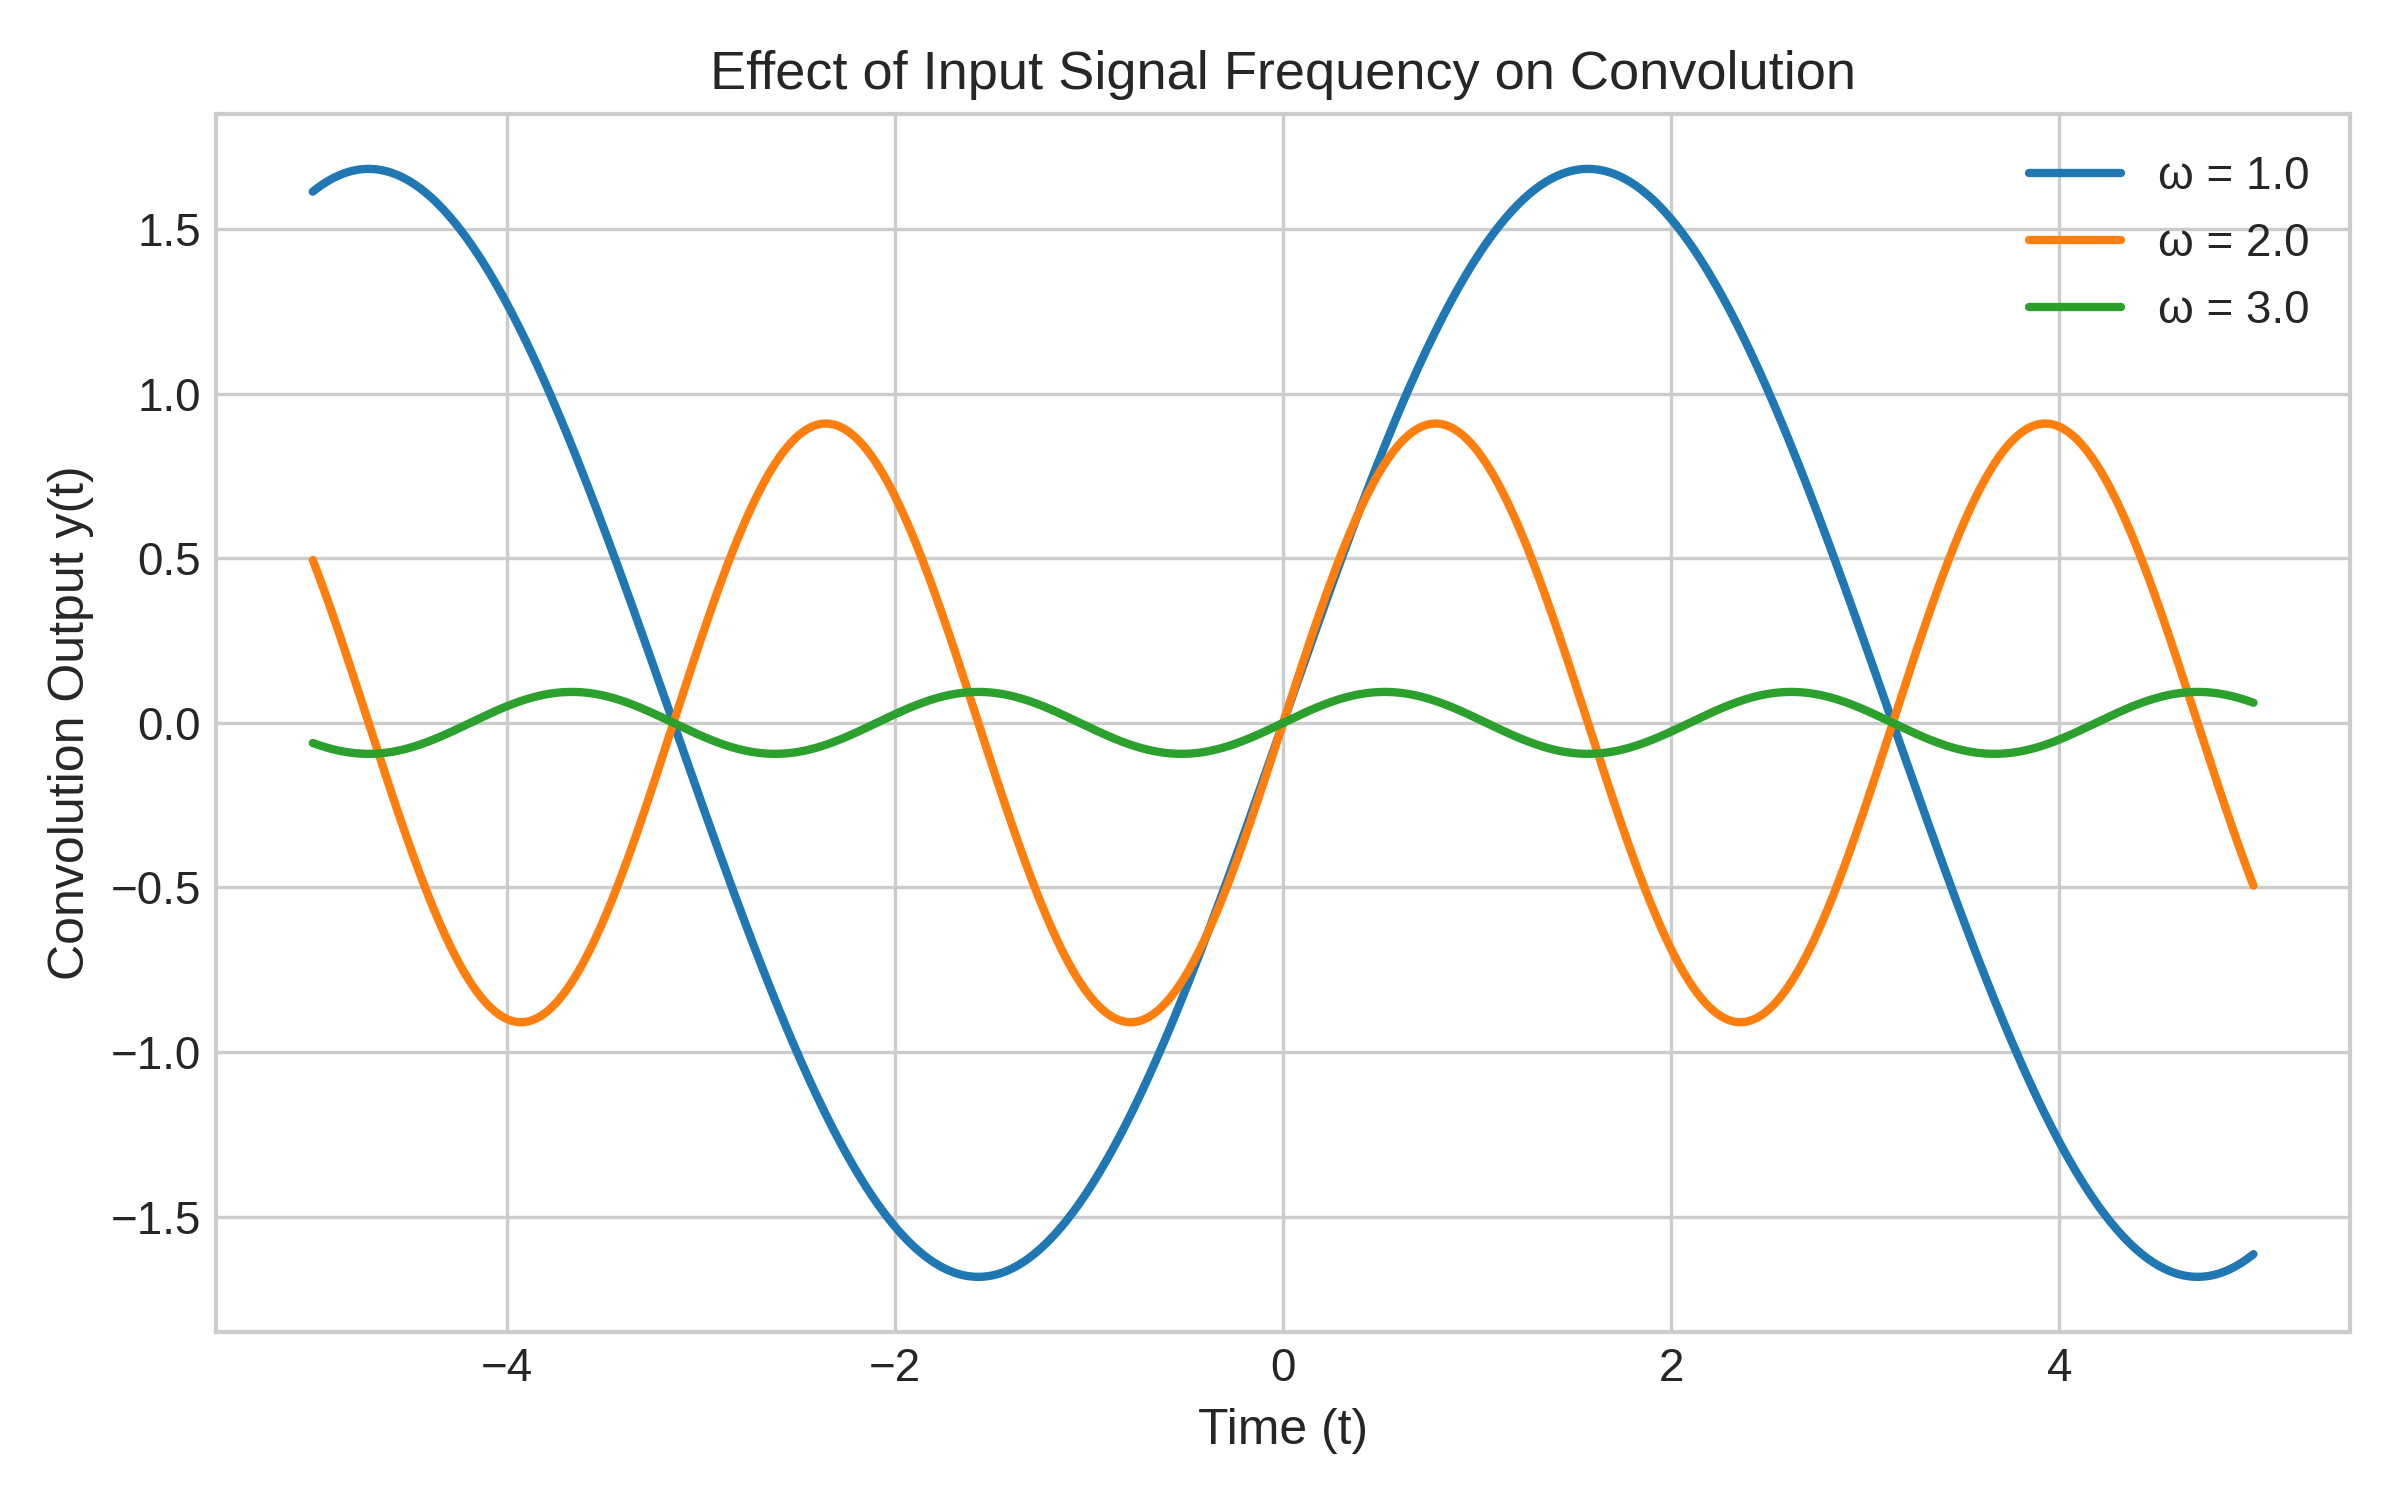
\includegraphics[width=0.8\textwidth]{codes/codes_sin_1_and_arcsin/figures/frequency_effect.png}
    \caption{Effect of varying input signal frequency on convolution output.}
    \label{fig:frequency}
\end{figure}

\subsubsection{Effect of Kernel Width}
The parameter $T$, which determines the kernel width, significantly impacts the convolution through the $\sin(\omega T)$ term in the amplitude factor. Figure \ref{fig:kernel} shows how different kernel widths affect the output.

\begin{figure}[H]
    \centering
    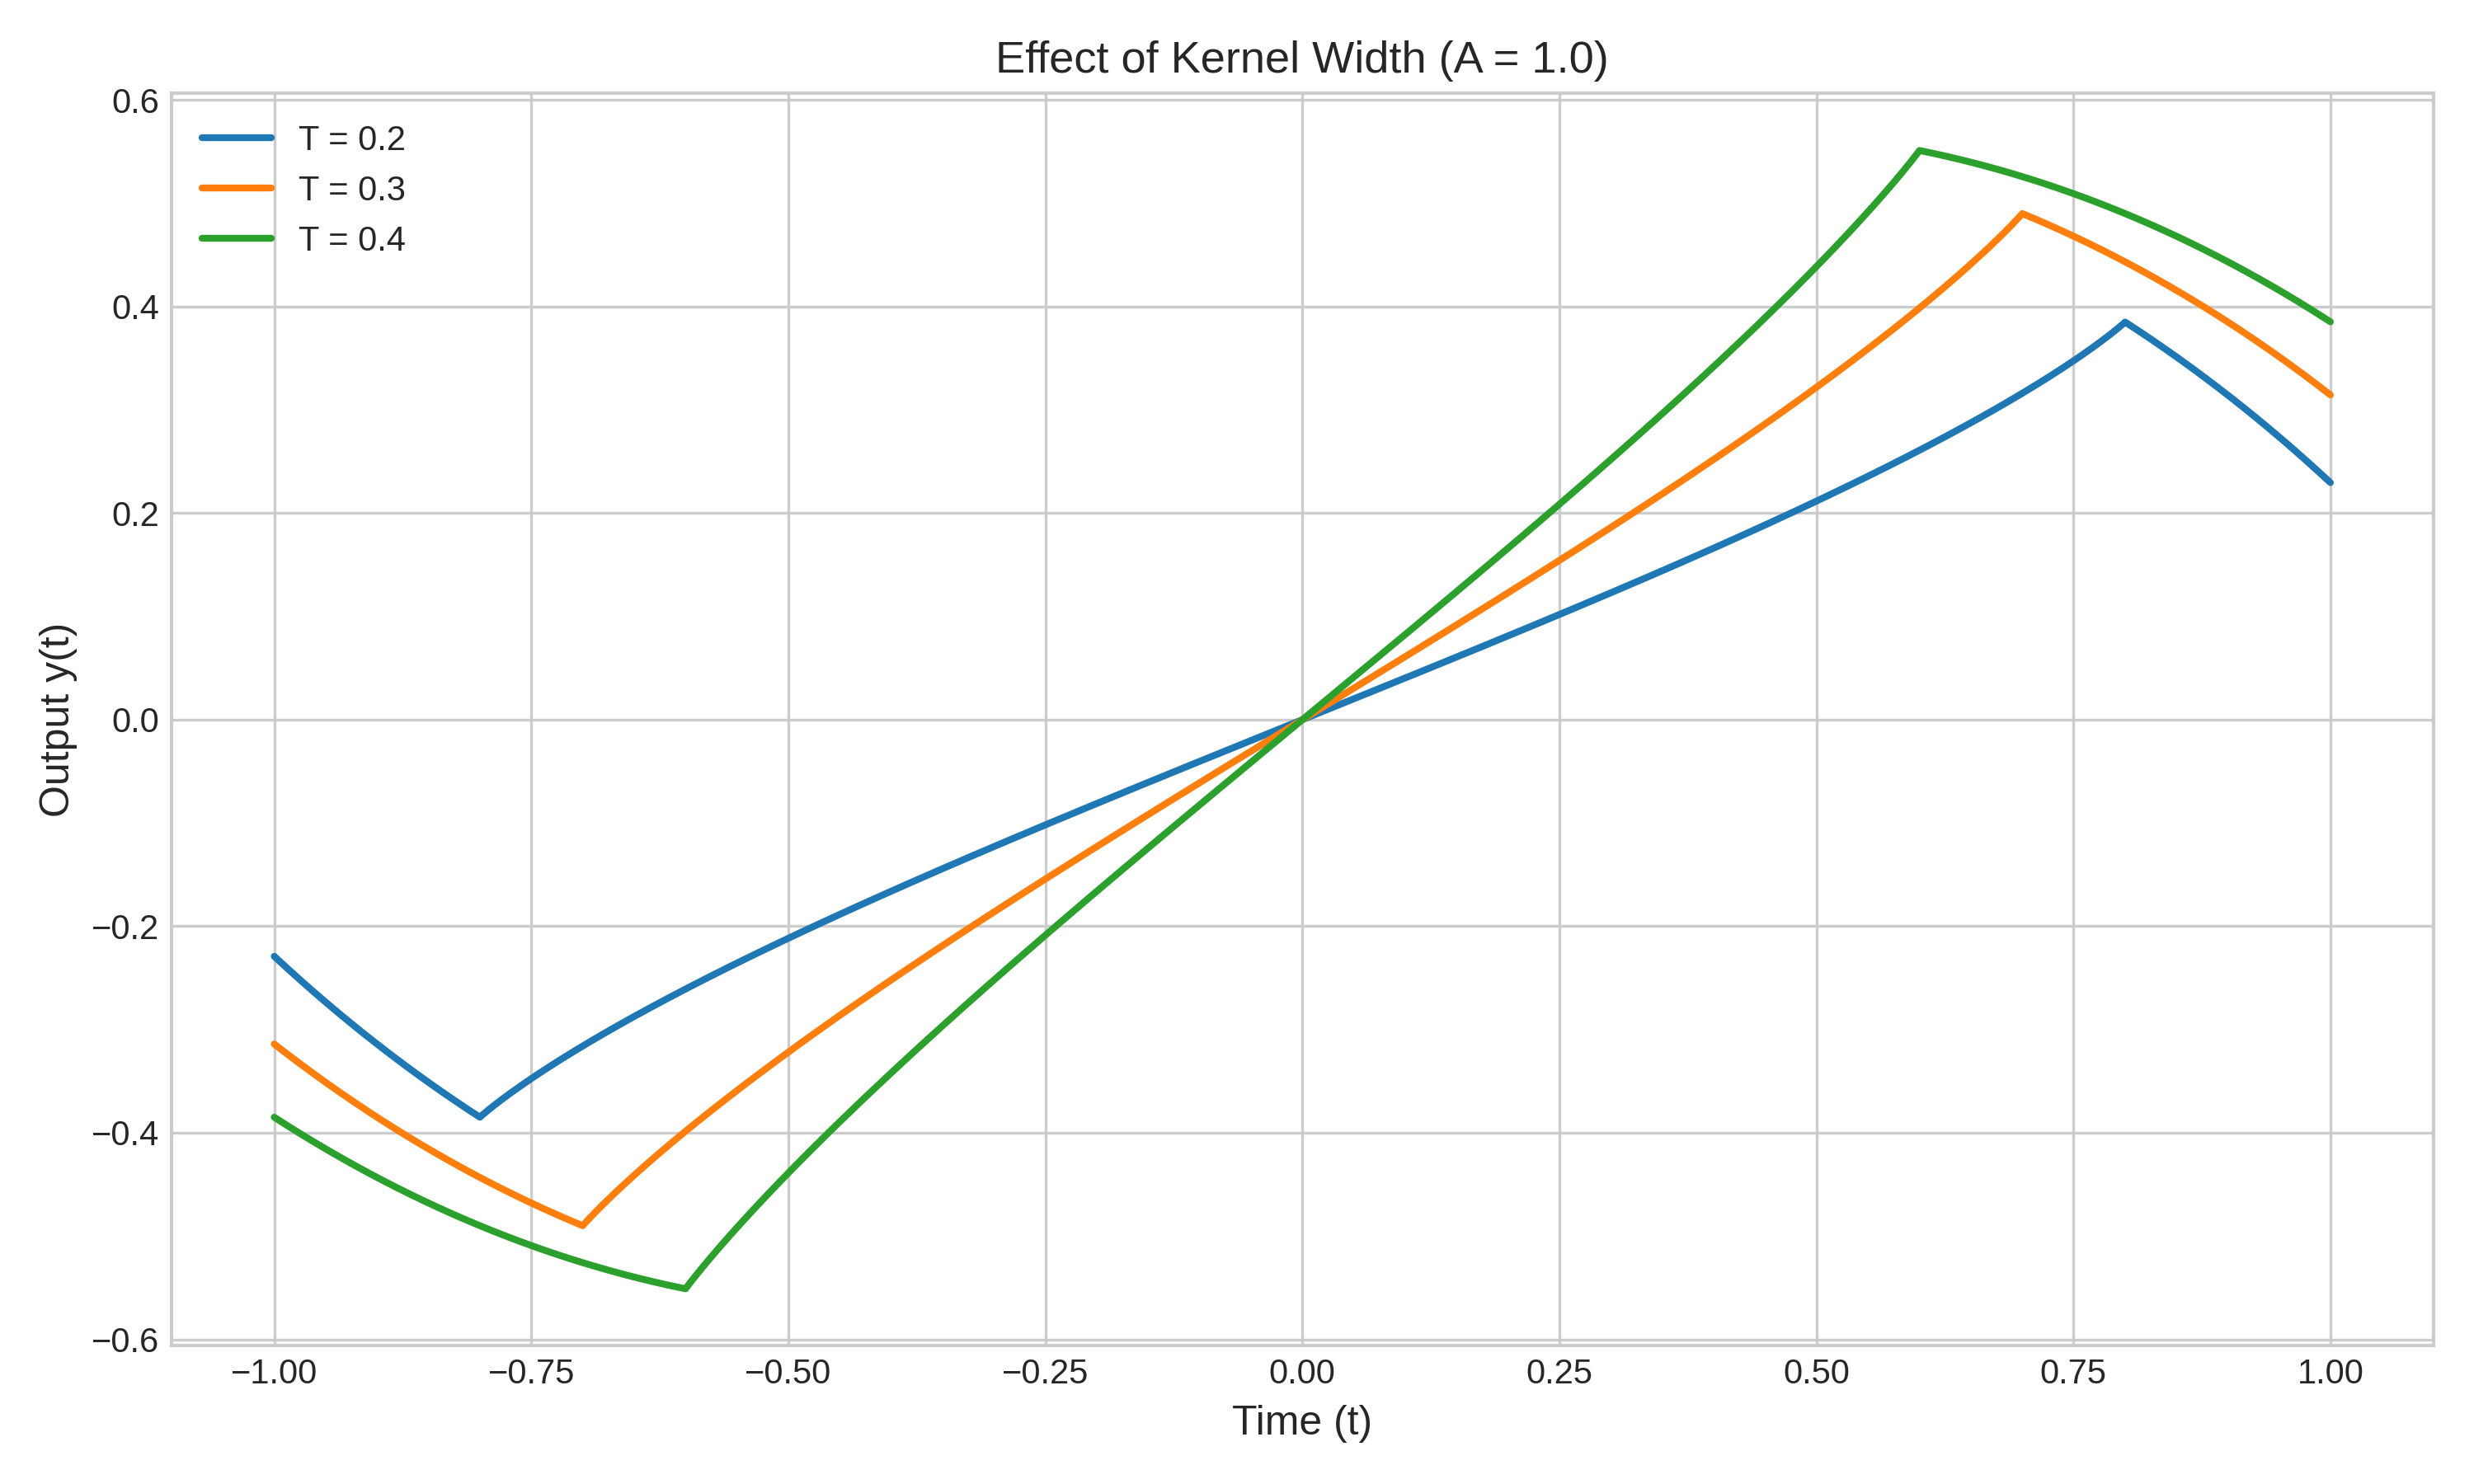
\includegraphics[width=0.8\textwidth]{codes/codes_sin_1_and_arcsin/figures/kernel_width_effect.png}
    \caption{Effect of varying kernel width on convolution output.}
    \label{fig:kernel}
\end{figure}


\subsection{Significance in Signal Processing}
These parameter dependencies reveal important practical implications:

\begin{itemize}
    \item The rectangular kernel acts as a frequency-selective filter, with the $\frac{2\sin(\omega T)}{\omega}$ term determining which frequencies pass through.
    
    \item The kernel width $T$ can be adjusted to target specific frequency ranges. Wider kernels (larger $T$) attenuate higher frequencies more strongly.
    
    \item The frequency nulls at $\omega T = n\pi$ demonstrate how certain combinations of input frequency and kernel width can completely eliminate signals.
    
    \item The system preserves the input signal's phase, which is important for maintaining signal timing relationships.
\end{itemize}

In practical applications, understanding these dependencies allows engineers to design appropriate filters for signal processing tasks or to predict how specific signal components will be affected by convolution operations.

\subsection{Conclusion}
The convolution of a sinusoidal signal with a rectangular kernel demonstrates key parameter dependencies that are fundamental to signal processing. The amplitude, frequency, and phase of the input signal, along with the kernel width, all influence the convolution output in specific ways. 

The most significant relationship is between the input frequency $\omega$ and kernel width $T$, which together determine whether signals are passed, attenuated, or completely nullified. This behavior forms the basis for filtering operations in many signal processing applications.
